\documentclass[tikz]{standalone}
\usepackage{amsmath, amssymb, amsfonts}
\usetikzlibrary {arrows.meta}
\usetikzlibrary {calc}
\begin{document}
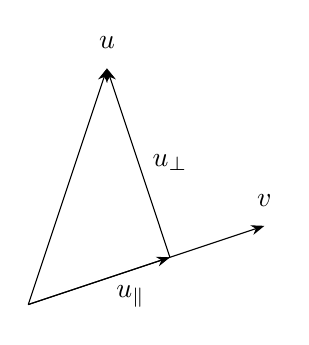
\begin{tikzpicture}[>=Stealth]
    \coordinate (o) at (0, 0);
    \coordinate (v) at (3, 1);
    \coordinate (u) at (1, 3);
    \coordinate (p) at ($(o)!(u)!(v)$);

    \draw[->] (o) -- (u);
    \draw[->] (o) -- (v);
    \draw[->] (p) -- (u);
    \draw[->] (o) -- (p);

    \node[shift={(-0.5,-0.5)}] (up) at (p) {$u_\|$};
    \node[shift={(+0.8,-1.2)}] (us) at (u) {$u_\perp$};
    \node[label=$u$] (u) at (u) {};
    \node[label=$v$] (v) at (v) {};
    % \node[point, label=$\mathfrak{m}s$] at (s) {};

    % \draw [->, thick] (f2) to [out=230, in=0]
    % node [below, sloped]  (m1) {$\mathfrak{m}_1$} (hs);
    % \draw [->, thick] (hs) to [out=230, in=0]
    % node [below, sloped]  (m1) {$\mathfrak{m}_2$} (h);
\end{tikzpicture}
\end{document}
